\chapter{Исследовательская часть}

\section{Технические характеристики}

Технические характеристики устройства, на котором выполнялся эксперимент:
\begin{itemize}
	\item операционная система: Ubuntu\cite{ubuntu} Linux x86\_64;
	\item память: 16 GiB;
	\item процессор: AMD Ryzen™ 7 4700U\cite{amd}.
\end{itemize}

\section{Проведение эксперимента}

Для каждого числа потоков было произведено 10 замеров процессорного времени, 
после чего определено среднее время выполнения алгоритма.

В таблице \ref{tab:profiling-1} представлены замеры процессорного времени (в мс)
для массива точек размера 2073600 (стандартное разрешение 1920 х 1080).

Результаты замеров представлены в табл. \ref{tab:profiling-1} и на рис. \ref{tab:profiling-1}.
\begin{table}[!ht]
	\begin{center}
		\captionof{table}{Время выполнения алгоритмов (в мс) для отсортированного массива}
		\begin{tabular}{|c|c|} 
			\hline
			Кол-во потоков & Время выполнения (мс) \\  
			\hline
			1 & 157.784 \\
			\hline
			2 & 86.275 \\
			\hline
			4 & 49.0306  \\
			\hline
			8 & 31.3017 \\
			\hline
			16 & 30.8065 \\
			\hline
			32 & 28.8583\\
			\hline
			64 & 27.9632 \\
			\hline
		\end{tabular}
		\label{tab:profiling-1}
	\end{center}
\end{table}

\begin{figure}[!h]
	\centering
	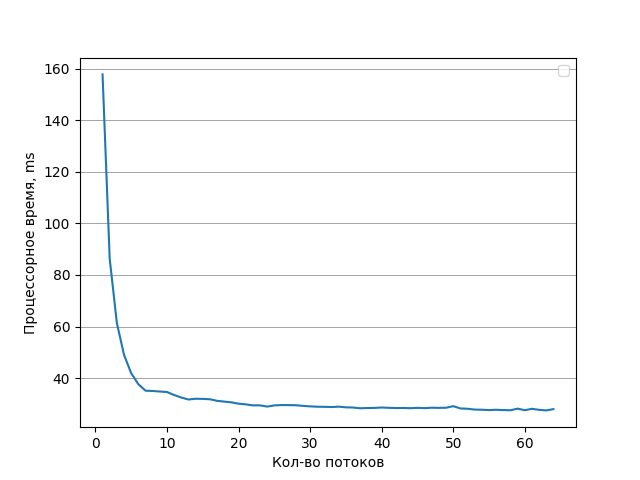
\includegraphics[scale=0.9]{imgs/measures_1.png}
	\caption{Зависимость времени работы алгоритма от кол-ва потоков}
	\label{img:profiling-1}
\end{figure}
\newpage


В таблице \ref{tab:profiling-2} и на рисунке \ref{tab:profiling-1} представлены замеры процессорного времени (в мс)
для ко­личества потоков, равного количеству логических ядер процессора.
\begin{table}[!ht]
	\begin{center}
		\captionof{table}{Замеры процессорного времени для кол-ва пото­ков, равного кол-ву логических ядер процессора}
		\begin{tabular}{|c|c|c|} 
			\hline
			Кол-во точек & Последовательный алгоритм & Параллельный алгоритм \\  
			\hline
			2000000 & 156.657 & 31.310 \\
			\hline
			1500000 & 113.098 & 24.814 \\
			\hline
			1000000 & 79.139 & 16.042 \\
			\hline
			500000 & 36.657 & 7.952 \\
			\hline
		\end{tabular}
		\label{tab:profiling-2}
	\end{center}
\end{table}

\begin{figure}[!h]
	\centering
	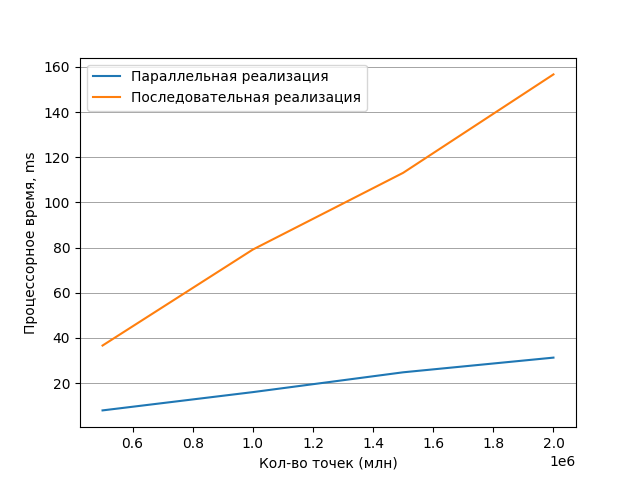
\includegraphics[scale=0.9]{imgs/measures_2.png}
	\caption{Зависимость процессорного времени от размерности массива (количество потоков равно 16)}
	\label{img:profiling-2}
\end{figure}
\newpage


\section{Вывод}

Из полученных выше результатов замеров процессорного време­ни можно сделать вывод,
что использование многопоточности однознач­но может дать существенной прирост 
эффективности. В данной лабора­торной работе в качестве примера рассматривался 
алгоритм поворота массива точек фигуры в пространстве, и при использовании 
много­поточности удалось добиться как минимум 6-кратного увеличения про­изводительности.

Даже при использовании двух потоков, вместо одонго, производительность увеличилась почти в
2 раза, однако при количестве потоков, равном количеству физических ядер (8 ядер), рост про­изводительности
начинает замедляться, а после количества потоков, равного 16 - столько логических ядер 
имеет процессор, время выполнения алгоритма практически стабильно.

Максимальное количество потоков, при которых выполнялись за­меры - 64
и при этом количестве производительность выросла в 6 раз, 
однако нельзя утверждать, что так будет всегда - если использовать слишком 
много потоков и часть данных для обработки в результате будет малой, то больше времени
бу­дет тратиться на создание и завершение потока, чем на обработку части
информации.

Также можно сделать вывод, что использовать 1 поток неэффек­тивно, 
т.к. по сути это эквивалентно обыкновенному последовательному
алгоритму, однако сверх этого тратятся ресурсы системы на создание и
закрытие потока, и в результате программа работает медленее.